% \documentclass[11pt, letterpaper]{article}
\documentclass{article}

\usepackage{algorithm2e}
\usepackage{graphicx}
\usepackage{natbib}
\usepackage{doi}
\usepackage{arxiv}
\usepackage{amsmath}
\usepackage{amsfonts}
\usepackage{amssymb}
\usepackage{bbm}
\usepackage{booktabs}
\usepackage{caption}
\usepackage{color}
\usepackage{diagbox}
\usepackage[shortlabels]{enumitem}
\usepackage{fancyhdr}
\usepackage[T1]{fontenc}
\usepackage{geometry}
\geometry{a4paper,scale=0.8}
\usepackage{graphicx}
\usepackage{fancyhdr}       % header
\graphicspath{ {./img/final}}
\usepackage{hyperref}
\usepackage{cleveref}  % cleverref must be imported after hyperref
\usepackage[utf8]{inputenc}
\usepackage{listings}
\usepackage{mathtools}
\usepackage{microtype}      % microtypography
\usepackage{multirow}
\usepackage{natbib}
\usepackage{nicefrac}
\usepackage{setspace}
\usepackage{url}
\renewcommand{\baselinestretch}{1}
\usepackage{lipsum}

% set-up header & footer
% \pagestyle{empty}
% \fancyhf{}
% \cfoot{\thepage}
% \lhead{%
% \textbf{University of California, Berkeley} \\
% Department of Elec. Eng. \& Comp. Sci.
% }
% \rhead{\textbf{CS 285 Deep Reinforcement Learning} \\Fall 2022
% }

\title{%
    Multi-Agent Reinforcement Learning for Assumption-Free Stock Market Modeling
}

\author{ \hspace{1mm}Maverick Zhang\\
	UC Berkeley\\
        Berkeley, CA 94720, United States \\
	\texttt{maverickzhang@berkeley.edu} \\
	%% examples of more authors
	\And
	\hspace{1mm}Juanwu Lu \\
	% Department of Civil and Environmental Engineering\\
	UC Berkeley \\
        Berkeley, CA 94720, United States \\
	\texttt{juanwu\_lu@berkeley.edu} \\
}
% Here you can change the date presented in the paper title
% \date{September 9, 1985}
% Or remove it
\date{}

% Uncomment to override  the `A preprint' in the header
% \renewcommand{\headeright}{Technical Report}
\renewcommand{\undertitle}{Technical Report}
% \renewcommand{\shorttitle}{\textit{arXiv} Template}
% \renewcommand{\undertitle}{}
\renewcommand{\headeright}{}

% \setlength{\headheight}{35pt}

%%% Add PDF metadata to help others organize their library
%%% Once the PDF is generated, you can check the metadata with
%%% $ pdfinfo template.pdf
\hypersetup{
    pdftitle={Multi-Agent Reinforcement Learning for Assumption-Free Stock Market Modeling},
    pdfsubject={q-bio.NC, q-bio.QM},
    pdfauthor={Maverick Zhang, Juanwu Lu},
    pdfkeywords={None},  % keyword
}

% % set-up code listing
% \definecolor{dkgreen}{rgb}{0,0.6,0}
% \definecolor{gray}{rgb}{0.5,0.5,0.5}
% \definecolor{manuve}{rgb}{0.58,0,0.82}

% \lstset{frame=tb,
%     language=Python,
%     aboveskip=3mm,
%     belowskip=3mm,
%     showstringspaces=false,
%     columns=flexible,
%     basicstyle={\small\ttfamily},
%     numbers=none,
%     numberstyle=\tiny\color{gray},
%     keywordstyle=\color{blue},
%     commentstyle=\color{dkgreen},
%     stringstyle=\color{manuve},
%     breaklines=true,
%     breakatwhitespace=true,
%     tabsize=3
% }

\begin{document}
\maketitle

% \thispagestyle{fancy}
% \pagestyle{plain}

\begin{abstract}
    %1 page extended abstract%
    Modeling consumer behavior in a market has long been an exciting challenge for economic research. A practical model can help predict and understand market behaviors and prevent fluctuations or unexpected breakdowns. However, existing modeling approaches either rely on restrictive assumptions or require complicated optimization procedures for online approximations. With recent progress in machine learning, deep reinforcement learning give rise to some state-of-the-art trading and forecasting techniques in economics. Nevertheless, more effort needs to focus on modeling the market behavior. This paper seeks to investigate building an assumption-free stock market model that depicts fine-grained individual decisions. A detailed stock market environment is proposed to incorporate multi-agent deep deterministic policy gradients (MADDPG) for modeling behaviors. Results from the experiments show that deterministic policy can result in the agents being trapped at a Nash Equilibrium.
    % \lipsum[1]
\end{abstract}

% keywords
\keywords{Stock Market Modeling \and Reinforcement Learning \and Multi-Agent Deep Deterministic Policy Gradient}

\section{Introduction}
Modeling behavior in a market is critical in economics, for all institutions: firms, households, and governments. Getting the model correct crucially allows preventative measures to be taken for the economy, especially when trying to prevent economic crises such as crashes or recessions. Since 2008, the market fragility hypothesis proposed by Hyman Minsky has been widely adopted \cite{minsky1992instability} as an explanation for why such large recessions have become commonplace. 

Subject to any shock, such as the COVID pandemic, we see the effects of market fragility such as runaway inflation; hence, it is an exciting challenge to build a model that may provide a more accurate prediction of the economy. To that end, a model should be sensitive and able to reflect individuals' choices with high fidelity and be largely assumption free. Since the development of macroeconomics, economic models have often needed to adopt extreme simplifying assumptions in order to be computationally feasible: leading to a problem in aggregation. Thus, while agent based modelling should be adopted (better predictions, but less deterministic and more computationally complex), most economic models in use for forecasting are based upon deterministic models derived from simplifying assumptions (simpler, deterministic, but are biased). Unfortunately, such models contributed to the 2008 recession, and flawed assumptions has historically prolonged economic disasters such as the Great Depression as well, a la Hooverism. 

Thus we seek to take first steps towards bridging this gap and develop a model that is computationally less complex, deterministic, and largely assumption free, taking multi agent reinforcement learning methods as our approach.

\section{Related Work}

\subsection{Aggregation Problem in Economics}
The aggregation problem is a well known problem that makes economics modeling hard. Due to complex interactions and emergent behavior, economic systems exhibit behavior that can be different on an aggregate and individual level, such as risk preference \citep{blackburn2008aggregation}. To deal with this, the microfoundations are abstracted away and forgotten, which reduces complexity enough to make economic systems modelable. In macroeconomics, the premier model is the Dynamic Stochastic General Equilibrium (DSGE) model \citep{gali2015monetary}. However, abstracting away the microfoundations restricts the modelling of emergent behavior. This can sometimes result in bad modelling predictions that have enormous consequences, such as the 2008 recession. 

The opposite approach to this type of modeling is Agent-based Computation Economics (ACE) models \citep{niazi2011ace} which seeks to begin with agents and keep the microfoundations, while being computationally expensive. But the benefit of ACE is that it can with minimal assumptions predict and exhibit emergent behavior.

\subsection{Reinforcement Learning for Economic Modelling}

Reinforcement learning (RL) is well-known for its ability to learn human-level control through experience-driven training. Figure 1 shows the basic logic that drives a reinforcement learning system. Progress in RL algorithms promotes its applications for modeling and understanding behaviors in complex systems, such as traffic flow \citep{lussange2021modelling}, human locomotion control \citep{song2021deep}, and many others. Existing literature has explored utilizing RL to help with forecasting and trading. Lee applied a temporal-difference algorithm in \citep{lee2001stock}, for daily stock price prediction. Compared with supervised learning, the algorithm is more robust for long-term prediction with delayed rewards. Sornmayura \citep{sornmayura2019robust} incorporated a DQN model trained on past historical data for foreign exchange price forecasting in its trading system. In \citep{ertuugrul2018forecasting}, generalized behavioral learning helped better forecast financial indicators on a 3-month basis. For automatic trading, Corazza and Sangalli compared Q-learning and SARSA for their applications in stock trading \citep{corazza2015q}. Carapuco et al. \citep{carapucco2018reinforcement} designed a system using classic reinforcement learning for foreign exchange trading. Conegundes et al. \citep{conegundes2020beating} demonstrated the power of Deep RL by beating the stock market in a day trading system. Nevertheless, reinforcement learning has yet to make its way into economics modeling \citep{tilbury2022rl}.

\begin{figure}[h]
\[ \begin{picture}(90,60)
  \put(25, 45){\framebox(30, 20){Agent}}
  \put(0, 0){\framebox(80, 20){Environment}}
  % Reward
  \put(0, 12){\vector(-1, 0){25}}
  \put(-25, 12){\line(-1, 0){5}}
  \put(-30, 12){\line(0, 1){40}}
  \put(-30, 52){\vector(1, 0){55}}
  \put(-10, 18){\makebox(0, 0)[c]{$r_{t+1}$}}
  \put(-25, 36){\makebox(0, 0)[l]{\ Reward $r_t$}}
  % State
  \put(0, 6){\vector(-1, 0){25}}
  \put(-25, 6){\line(-1, 0){15}}
  \put(-40, 6){\line(0, 1){52}}
  \put(-40, 58){\vector(1, 0){65}}
  \put(-10, 0){\makebox(0, 0)[c]{$s_{t+1}$}}
  \put(-40, 36){\makebox(0, 0)[r]{State $s_t$\ }}
  % Action
  \put(55, 55){\line(1, 0){55}}
  \put(110, 55){\line(0, -1){45}}
  \put(110, 10){\vector(-1, 0){30}}
  \put(105, 36){\makebox(0, 0)[r]{Action $a_t$\ }}
\end{picture}
 \]
\caption{The interaction between agent and environment in reinforcement learning.}
\label{fig:1}
\end{figure}

Before this work, Lussange et al. \citep{lussange2021modelling} explored modeling stock markets with multi-agent reinforcement learning in their paper. However, the model is trained on a daily trading basis, an aggregation over temporal dimension that may fail to capture minor fluctuations in buyers' decisions. Instead, in our model, we allow agents to trade every 5 minutes under clearance, which fits the settings of a real stock market. We will cover more details on our environment in the following section.

\section{Methodology}
% Our approach is a compromise between the DSGE model and ACE model approach. To avoid the extreme computational drawbacks of a full economy with millions of agents, we will use macroagents that are intended to imitate sectors or groups of agents in the economy. For example, we might have agents that are stratified by wealth, give rich agents a higher budget as opposed to poor agents. However, rather than following DSGE models and imposing rules, other than giving the agents rewards or punishments, we allow them to interact with an economic system how they like to maximize their rewards. Then we apply multi-agent reinforcement learning to observe behavior. This way we can still obtain emergent behavior and get rid of assumptions, while preventing the complexity from blowing up. We could even investigate problems such as market fragility by observing changes to the system with more or less agents. 
This paper aims to build a stock market model between the DSGE and ACE models, where we incorporate multi-agent deep reinforcement learning to learn the behaviors of agents in a stock market directly via interactions to reduce online optimizations seen in ACE models while not abstracting the microfoundations as seen in DSGE models. In this section, we present detailed settings of the stock market environments, along with the multi-agent deep deterministic policy gradients (MADDPG) we used to learn agents' behaviors. Compared to the classic models, our proposed model can obtain emergent behavior without assumptions and prevent the complexity from blowing up.

\subsection{Stock Market Environment}
% The environment we chose to use was a stock market environment. Internally, we provide several agents a starting budget and a stock with which they can sell or buy shares of to make more profit.

\subsubsection{Agents, Market, and Trading System}

Instead of modeling a colossal system with millions of agents, our model uses macro agents intended to imitate sectors or clusters of populations in the economy. For instance, populations in real life may be stratified by wealth and the ability to know latent information within a market. Therefore, in our environment, we initialize agents with different initial funding, shareholdings, and masks of available information. These agents are driven by an intuitive objective, maximizing the final amount of money for each environment episode. Each episode of the environment lasts 390 timesteps, corresponding to the total daily trading minutes in a real stock market. Each deal agents make must go through a clearance procedure, where a queue holds and randomly assigns bidders and sellers for buying and selling their holdings. This process is shown in Algorithm 1.

\begin{algorithm}[hbt!]
\caption{The clearance procedure}\label{algo:1}
\KwData{ Agent price proposals and quantities $(p_1, q_1), \ldots, (p_n, q_n)$}
\KwResult{Returns $\Delta S$ and $\Delta B$ made per agent}
 buyers $:= \{i \mid q_i > 0\}$\;
 sellers $:= \{i \mid q_i < 0\}$\;
 $(\Delta S_i, \Delta B_i) = (0, 0)$ for all $i \leq n$\;
 randomize(buyers)\;
 randomize(sellers)\;
 \While{buyers $\neq \emptyset$ and sellers $\neq \emptyset$}{
  b $\in$ buyers\;
  s $\in$ sellers\;
  
  \eIf{$p_b \geq p_s$}{
   $\Delta B_b = \Delta B_b - p_b \cdot q_b$\;
   $\Delta S_b = \Delta S_b + q_s$\;
   $q_b = q_b - q_s$\;
   $\Delta B_s = \Delta B_s + p_s \cdot q_s$\;
   $\Delta S_s = \Delta S_s - q_s$\;
   $q_s = q_s + q_b$\;
   }{
   \textbf{continue}\;
  }
  \If{$q_b$ = 0}{
    delete b from buyers\;
  }
  \If{$q_s$ = 0}{
    delete $s$ from buyers\;
  }
 }
\end{algorithm}

\subsubsection{State}
Their interactions in the market determine the price of a stock and therefore the worth of their shares held. In addition, to give them information about their fellow competitors in the market, we provide stocks that change based upon the volatility of the agents bids and asks. In addition, we provide dummy stocks that change according to Brownian motion that are independent of the volatility. This way each agent can obtain a very noisy estimate of their opponents. In addition, we mask out some of the stocks depending on the agent. That is, not all agents are focused on all the stocks and may get noisier or less noisy estimates of their competitor's actions. 

The state is therefore:
\begin{equation}
    s_t = (P_t, \mathbf{c}_t, \mathbf{u}_t, M, B_t, S_t)
\end{equation}
where $P_t$ is the current price of the stock, $\mathbf{c}_t$ is the vector of correlated stocks, $\mathbf{u}_t$ is the vector of uncorrelated stocks (Brownian motion), $M$ is a mask vector to determine which stocks are being considered by an agent, $B_t$ is the money held by the agent (real assets), and $S_t$ is the shares held by the agent (financial assets)

\subsubsection{Action}
Agents can either bid or sell an asset, and they can determine the price they are willing to sell. We implement limit transactions and only allow a transaction to proceed if another agent is willing to make the deal. Now the agent therefore has a two dimensional action
\begin{equation}
    a_t = (p_t, q_t)
\end{equation}
where $p_t$ is the price of a bid or ask, and $q_t$ is the quantity of shares to buy (positive) or sell (negative). 

\subsubsection{Rewards}

Their rewards simply their real assets and their financial assets summed. We provide an environment parameter $\omega$ that determines the relative importance of shares held vs. money. We also place a decay on the real assets currently held by an agent ($\gamma$) so agents are incentivized to enter the market and not hold. In addition, we must have the current stock price in order to convert shares held into a common unit. Thus, our rewards are 
\begin{equation}
    r(s_t, a_t) := \omega S_tP_t + B_t
\end{equation}
where the assets at each time step

\subsection{Multi-Agent Deep Deterministic Policy Gradient}
We use Multi-Agent Deep Deterministic Policy Gradient (MADDPG) \citep{lowe2017maddpg}, a commonly used multi-agent reinforcement learning algorithm to try and learn our economic model. The critical insight of MADDPG is the centralized-training-decentralized execution structure, where agents' Q-functions utilize the global state and actions from other agents to stabilize the training. We argue that this setting holds for real-world situations since many of the trading platforms would allow bidders to view others' bids.

For our implementations, each agent is represented by a policy network $\mu^{\theta}(a_t|s_t)$, and a critic network $Q^\phi(s_t, a_t)$. Both are three-layer MLP with 64 neurons each layer. Models are trained on a learning rate of 0.0001 and a reward discount factor of 0.99. Algorithm 2 shows the training procedure of MADDPG.

\begin{algorithm}
    \caption{Multi-Agent Deep Deterministic Policy Gradient \citep{lowe2017maddpg}}\label{algo:2}
    \KwData{Batch size $S$; Reward discount $\gamma_r$; Replay buffer $\mathcal{D}$; Number of agents $N$; Total number of episodes $M$; Random process $\mathcal{N}$ for exploration; Episode index $i=0$.}
    \While{$i<M$}{
        Initialize the random process $\mathcal{N}$
        Receive initial state $s$
        \While{not \textit{done}}{
            for each agent $i$, select action $a_i=\mu^{\theta_i}(o_i)+\mathcal{N}_t$ w.r.t the current policy and exploration;
            
            Execute action $a=(a_1,\ldots,a_N)$, observe reward $r(s, a)$ and new state $s^\prime$;
            
            Store transition $(s, a, r, s^\prime$ in replay buffer $\mathcal{D}$;
            
            $s\leftarrow s^\prime$;
            
            Initialize agent index $j=1$;
            
            \While{$j<N$}{
                Sample a random mini-batch of $S$ samples $(s^j, a^j, r^j, s^{\prime j}) from \mathcal{D}$;
                
                Set $y^j = r_i^j + \gamma\left.Q_i^{\phi^\prime}(s^{\prime j},a_1\prime, \ldots, a_N^\prime)\right|_{a_k^\prime=\mu_k^\prime(o_k^j)}$;

                Update critic by minimizing Bellman-error $\mathcal{L}(\phi_i)=\frac{1}{S}\sum_j\left(y^j-\left.Q_i^{\phi}(s^j,a_1^j,\ldots,a_N^j)\right|_{a_i=\mu_i(o_i^j)}\right)$;

                Update actor using the sampled policy gradient:
                \begin{equation*}
                    \nabla_{\theta_i}J\approx\frac{1}{S}\sum_j\nabla_{\theta_i}\mu_i(o_i^j)\nabla_{a_i}\left.Q_i^{\phi_i}(s^j,a_1^j,\ldots,a_N^j)\right|_{a_i=\mu_i(o_i^j)}
                \end{equation*}
                
                $j\leftarrow j+1$;
            }
            Update target network parameters for each agent $i$:
            \begin{equation*}
                \theta_i^\prime\leftarrow \tau\theta_i+(1-\tau)\theta_i^\prime
            \end{equation*}
            
            $i\leftarrow i+1$;
        }
    }
\end{algorithm}

\section{Experiment}

\subsection{Environment Settings and Training}
% \begin{table}[t!]
% \centering
% \caption{Final amount of money for all environment agents with different hyperparameter and action settings.}
% \begin{tabular}{@{}cccccccc@{}}
% \toprule
% \multicolumn{2}{c}{\multirow{2}{*}{\textbf{Hyperparameter}}}           & \multicolumn{3}{c}{\textbf{Budget Discount}}  & \multicolumn{3}{c}{\textbf{Weight of Stock}}  \\ \cmidrule(l){3-8} 
% \multicolumn{2}{c}{}                                                   & \textbf{0.50} & \textbf{0.90} & \textbf{0.95} & \textbf{0.10} & \textbf{0.50} & \textbf{0.90} \\ \midrule
% \multirow{5}{*}{\textbf{Trade on All or Nothing}}   & \textbf{Agent 1} & 307.56        & 1216.07       & 963.19        & 1276.40       & 593.93        & 820.26        \\
%                                                     & \textbf{Agent 2} & 730.29        & 1865.86       & 592.20        & 1977.16       & 1027.46       & 913.33        \\
%                                                     & \textbf{Agent 3} & 1590.94       & 709.20        & 1662.35       & 405.65        & 1867.00       & 1931.56       \\
%                                                     & \textbf{Agent 4} & 1695.38       & 1158.35       & 1025.33       & 1449.68       & 469.25        & 1789.77       \\
%                                                     & \textbf{Agent 5} & 1785.97       & 2092.91       & 1445.26       & 1055.45       & 611.71        & 1911.09       \\ \midrule
% \multirow{5}{*}{\textbf{Trade with Share Quantity}} & \textbf{Agent 1} & 713.02        & 1627.01       & 925.24        & 1826.60       & 709.73        & 290.40        \\
%                                                     & \textbf{Agent 2} & 1000.33       & 381.05        & 1348.52       & 51.20         & 696.49        & 1592.50       \\
%                                                     & \textbf{Agent 3} & 1002.54       & 775.53        & 1530.22       & 1343.31       & 973.13        & 1936.94       \\
%                                                     & \textbf{Agent 4} & 1119.39       & 1992.25       & 906.40        & 1095.31       & 209.98        & 1583.59       \\
%                                                     & \textbf{Agent 5} & 2065.37       & 935.72        & 847.57        & 1898.08       & 1997.82       & 506.02        \\ \bottomrule
% \end{tabular}
% \end{table}

% final budgets info: 
% all or nothing, budget = 0.50:  307.55592939  730.29170392 1590.94291925 1695.38462257 1785.96908467
% all or nothing, budget = 0.90: 1216.06515933 1865.86497511  709.19873799 1158.35152093 2092.90680078
% all or nothing, budget = 0.95: 963.19438551  592.20414851 1662.34702079 1025.32995434 1445.25825837
% all or nothing, worth of stocks = 0.10: 1276.40271882 1977.16232242  405.65248943 1449.68234277 1055.4540957
% all or nothing, worth of stocks = 0.50: 593.93318993 1027.46417776 1866.99902435  469.2546945   611.70703133
% all or nothing, worth of stocks = 0.90:  820.26425713  913.33378863 1931.56014156 1789.7702699  1911.09005057

% quantity setting, budget = 0.50: 713.01494521 1000.33111442 1002.53657601 1119.38914947 2065.37312019
% quantity setting, budget = 0.90: 1627.00856895  381.05407292  775.53306128 1992.2529543   935.71896846
% quantity setting, budget = 0.95: 925.23781906 1348.51807794 1530.22470238  906.394523    847.57291307
% quantity setting, worth of stocks = 0.10: 1826.59616464   51.19506377 1343.30499955 1095.30516363 1898.08499507
% quantity setting, worth of stocks = 0.50:709.72857832  696.4923973   973.12589219  209.9826533  1997.81863528
% quantity setting, worth of stocks = 0.90: 290.39814004 1592.50428855 1936.94444647 1584.59197313  506.01481712

To facilitate our investigation into agents' trading strategies, we compared results trained with four groups of hyperparameter and action settings, including different budget discounts ($\gamma$), worth of stock ($\omega$), an action space with share quantity, and an action space applied all or nothing rule. As mentioned in 3.1.4, a budget discount is analogous to the inflation rate in real life and acts as incentive for agents to enter the market. Generally, mild inflation can increase stock trading, while hyperinflation decreases it. The worth of stock is a ratio factor, which indicates how much an agent would treasure its stock holdings against its cash. We run our training on two market rules, one with the "all or nothing" rule, which means an agent has to sell all his shares or sell nothing, whereas the other allows agents to decide the quantity to buy or sell. Debts are not allowed in our environment, meaning any agent with its current amount of cash below 0 would terminate the episode.
Results from all our experiments are shown in Figures 2-5.

\begin{figure}[h!]
    \centering
    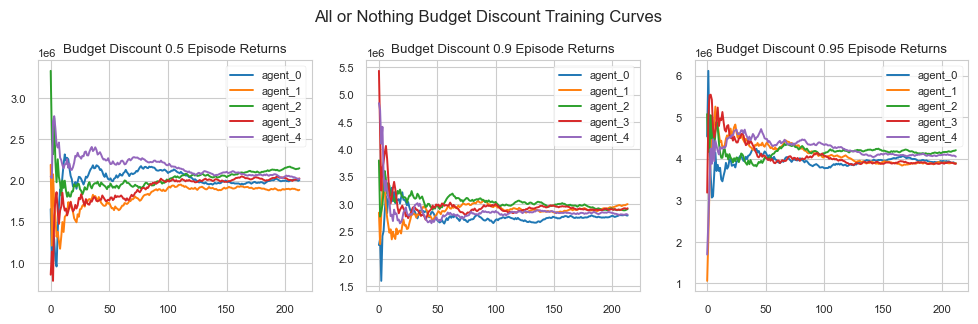
\includegraphics[width=0.90\textwidth]{all_or_nothing_budget.png}
    \caption{Episode total returns with a budget discount over time of 0.50 (left), 0.90 (middle), and 0.95 (right) when agents trade on all or nothing.} % Add here
    \label{fig: 2}
\end{figure}

\begin{figure}[h!]
    \centering
    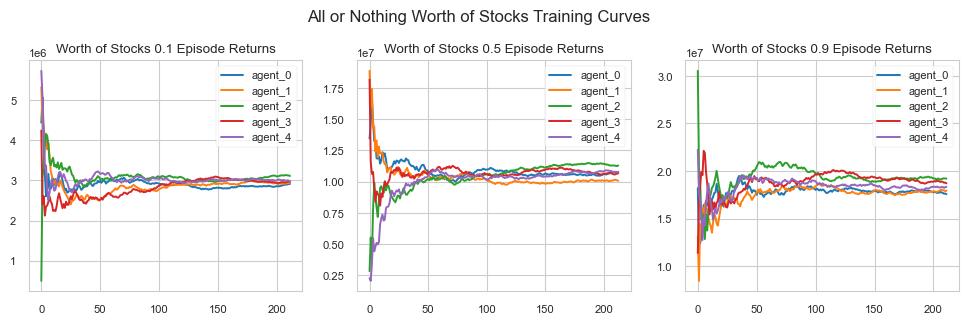
\includegraphics[width=0.90\textwidth]{all_or_nothing_stocks.png}
    \caption{Episode total returns with a worth of stock of 0.10 (left), 0.50 (middle), and 0.90 (right) when agents trade on all or nothing.} % Add here
    \label{fig: 3}
\end{figure}

Training curves from all our experiments are shown in Figures 2-5. Overall, the curves demonstrate similar patterns, where agents start with competing and aggressive strategies, causing episodic return oscillations. By the end of the training, agents from the same experiment settings will have their episode total returns stabilized at approximately the same level. The difference in episodic returns' scale is affected by random initialization and budget discount factors.

\begin{figure}[h!]
    \centering
    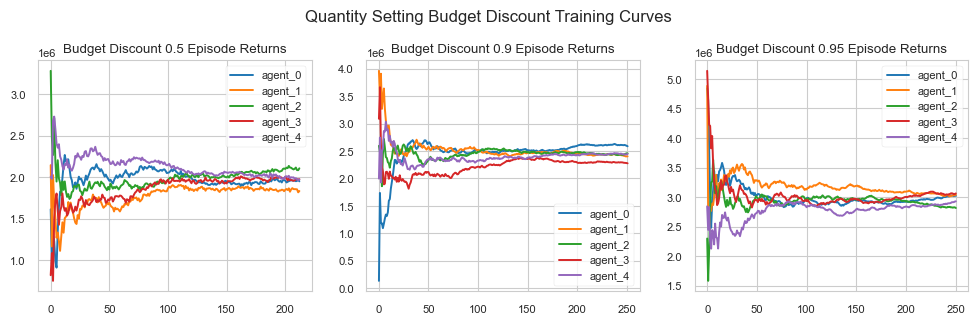
\includegraphics[width=0.90\textwidth]{quantity_setting_budget.png}
    \caption{Episode total returns with a worth of stock of 0.10 (left), 0.50 (middle), and 0.90 (right) when agents trade with share quantities.} % Add here
    \label{fig: 4}
\end{figure}

\begin{figure}[h!]
    \centering
    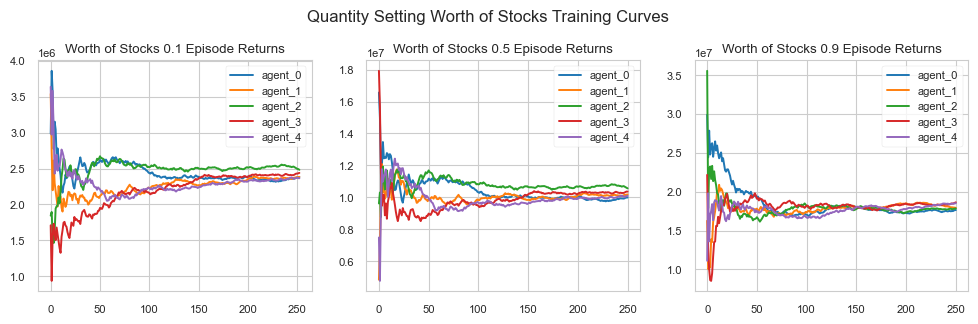
\includegraphics[width=0.90\textwidth]{quantity_setting_stocks.png}
    \caption{Episode total returns with a worth of stock of 0.10 (left), 0.50 (middle), and 0.90 (right) when agents trade with share quantities.} % Add here
    \label{fig: 5}
\end{figure}

The convergence of episodic total returns can usually be associated with equilibrium, where agents consent to take conservative actions for either selfish reasons or the public good. We further investigate the potential causes for the convergence in our results and explain from the perspective of Nash Equilibrium in the following sections.




% strategies
\subsection{Underestimation of Q Values}
Given that all the agents, in both problem settings and across a wide range of hyperparameters converge upon the same strategy: hold their shares, this suggests some system wide issue prevalent within our approach. Figure 6 shows the Q-values against the actual returns (dashed lines). We find that there is a systematic underestimation of Q-values, with the actual return far higher 

Furthermore, each agent seems to have converged to a similar critic function, just at different scales. This suggests the agents perceive the same actions lead to the same level of reward. In other words they have adopted the same strategy, and one that is overly pessimistic.

\begin{figure}[h!]
    \centering
    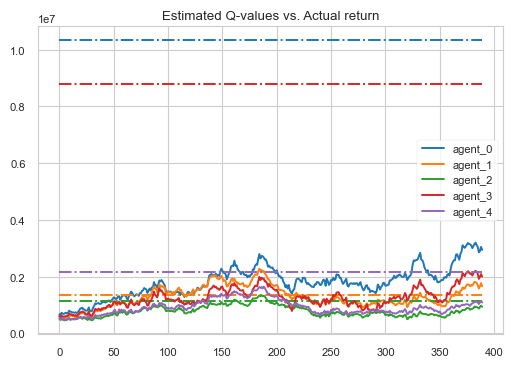
\includegraphics[width=0.6\textwidth]{img/final/q_values.png}
    \caption{Q-values for one episode. Above is the quantity setting, worth of stocks = 0.90 model. All other models were similar. Dotted lines are agent's actual return}% Add here
    \label{fig: 6}
\end{figure}

\subsection{Nash Equilibrium and Determinism}
It seems the deterministic nature of MADDPG and the centralized critic function led to a Nash Equilibrium that all the models converged to. Since the critic is centralized, the actor trains to find the best strategy while considering the strategy of all the other agents held constant. That is, the agent tries to improve its strategy until it can't anymore, while all other agents do the same. They all reach a strategy whereby they all try to buy in order to acquire more stocks to later sell. But upon reaching this strategy, all the agents are stuck due to the deterministic policy. They all seek to buy in order to acquire more value, but the deterministic policy means they cannot randomly try another action but their best perceived one, buying. Furthermore, they cannot improve their strategy: if any agent chooses to sell instead of buy, then the remaining agents can thereafter sell or sit on the shares bought to accumulate value, and now the agent that has sold its shares is at a disadvantage. They have arrived at a Nash Equilibrium. Knowing the strategies of the other players, and treating the strategies of the other players as set in stone, no agent can benefit by changing their strategy.

\section{Conclusion}
The agent based economic modelling approach is a promising one that may allow economists to bridge the gap in the aggregation problem. Many have, in this agent based approach, naturally tried to apply reinforcement learning in limited settings, such as abstracting away shares to be traded. However, two problems are still present in agent based approaches: computational complexity and determinism. Trying to limit the stochasticity of these models appears to in fact be impossible. The deterministic policies from reinforcement learning, while powerful, do not do well in such a complex environment, and can result in the agents getting stuck at a nash equilibrium. 

\bibliographystyle{unsrtnat}
\bibliography{reference}


\end{document}